% sec_balance.tex
\section{Баланс импульса на границе}

Рассмотрим движение частиц вихревого объекта в системе отсчёта, связанной с его центром симметрии. Так как это вихревой тороид, его центр симметрии является центром масс объекта, а согласно \textbf{теореме Кёнига} в системе центра масс геометрическая сумма импульсов Амеров, составляющих вихревой объект, равна нулю. Это означает, что для каждой частицы вихревого потока, обладающей импульсом, существует частица с импульсом, равным по величине, но противоположно направленным. Столкновения частиц внутри потока в процессе направленного движения не изменяют величину суммарного импульса такой системы ввиду её замкнутости, но такое изменение возможно через соударения с частицами Свободного эфира на внешней границе. Через граничную поверхность вихревого эфирного тороида одновременно протекают два потока импульса: один \(P^{+}\) из Свободного эфира внутрь вихревого эфирного тороида, другой \(P^{-}\) в обратном направлении. Физический и смысловой интерес представляет разность величин этих потоков \(\Delta P = P^{+} - P^{-}\), позволяющая установить связь между кинетическими параметрами акторов осуществления вихревых эфирных объектов весомой материи и сформулировать \textbf{условия} и \textbf{критерии} существования такого процесса.

%\begin{figure}[h]
%\centering
%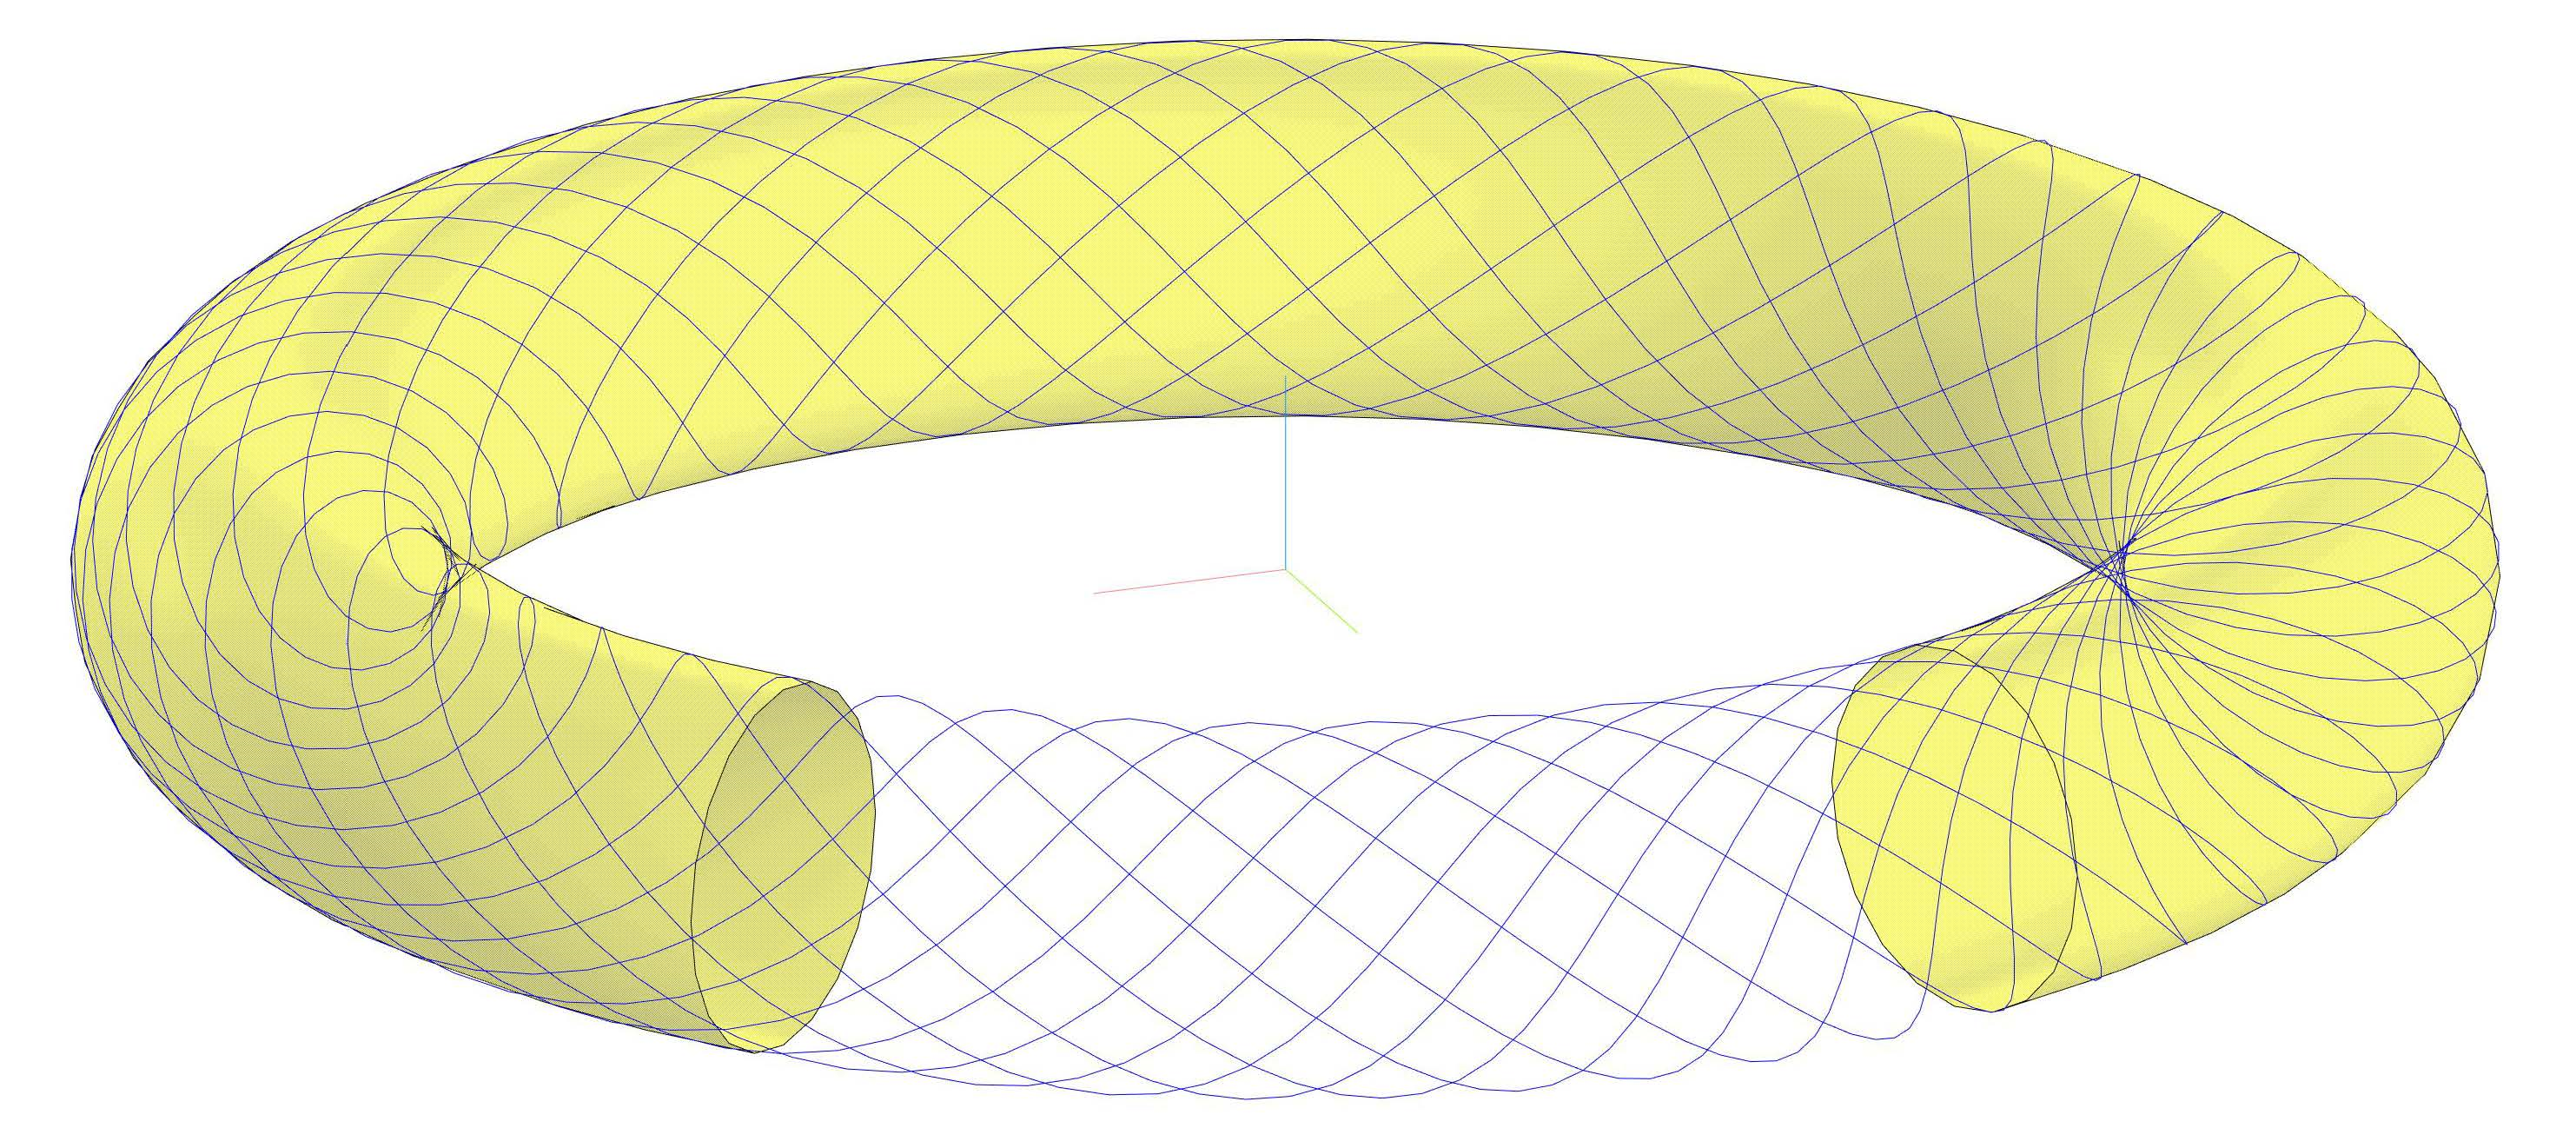
\includegraphics[width=0.4\textwidth]{images/a22.png}
%\caption{Условная поверхность раздела.}
%\label{fig:surface}
%\end{figure}

Акт абсолютно упругого соударения Амеров в системе отсчёта, связанной с точкой их касания при ударе, где одна из осей коллинеарна линии, соединяющей центры Амеров (рис. \ref{fig:collision1}, ось \(X\)), предполагает «обмен» компонентами импульсов, направленными вдоль этой оси координат. В дальнейшем линию, соединяющую центры соударяющихся Амеров и проходящую через точку их касания при ударе, будем называть \textbf{«осью соударения»}. Равенство масс сталкивающихся частиц делает возможным такой же «обмен» для аналогичных компонент скоростей до и после столкновения:

\[
m_a \mathbf{v}_1 + m_a \mathbf{v}_2 = m_a \mathbf{v}_1' + m_a \mathbf{v}_2' \;\Longrightarrow\; \mathbf{v}_1 + \mathbf{v}_2 = \mathbf{v}_1' + \mathbf{v}_2'.
\]

%\begin{figure}[h]
%\centering
%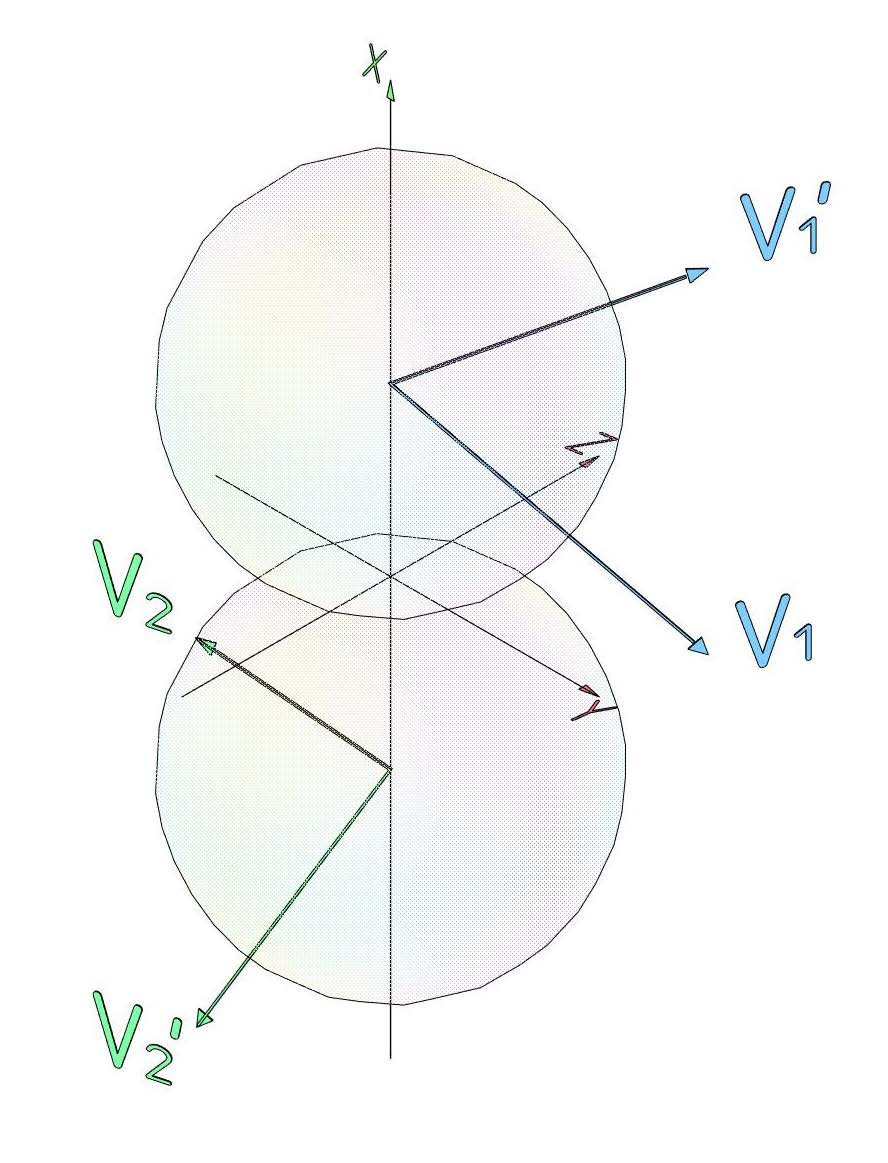
\includegraphics[width=0.3\textwidth]{images/a11.png}
%\caption{Схема столкновения двух Амеров (3D).}
%\label{fig:collision1}
%\end{figure}

%\begin{figure}[h]
%\centering
%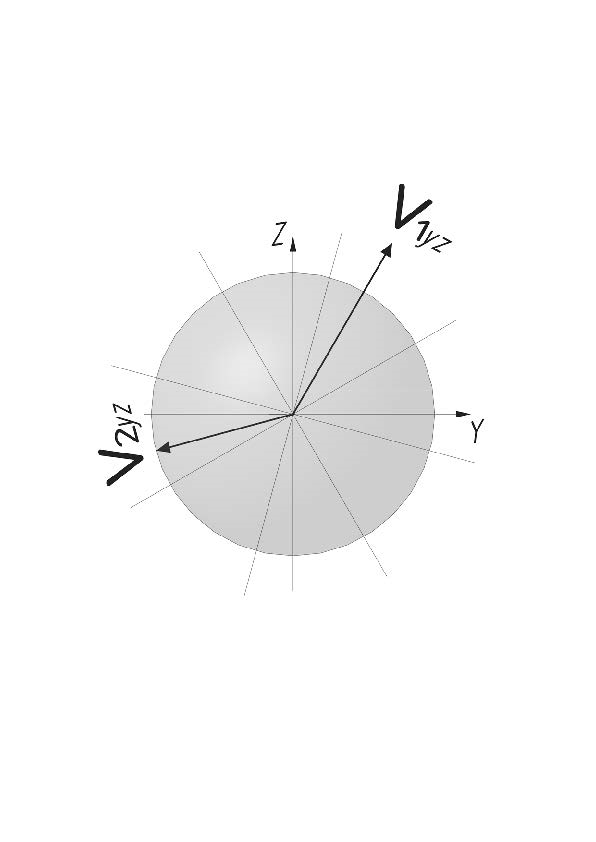
\includegraphics[width=0.4\textwidth]{images/a9.png}
%\caption{Вид вдоль оси соударения.}
%\label{fig:collision2}
%\end{figure}

На рис. \ref{fig:collision1} изображена трёхмерная модель столкновения двух Амеров в системе отсчёта, связанной с точкой их касания при абсолютно упругом соударении. На рис. \ref{fig:collision2} то же самое со стороны оси \(X\) (сверху) и \textbf{оси соударения}. Индекс «\('\)» обозначает состояние Амеров \textbf{после} акта соударения. Как видно из рис. \ref{fig:collision1}, «обмен» \(V_{1X}\) на \(V_{2X}\) для одного Амера и \(V_{2X}\) на \(V_{1X}\) для другого после соударения существенно изменил первоначальную физическую картину: столкнувшиеся Амеры стали разлетаться. При этом на виде, приведённом на рис. \ref{fig:collision2}, никаких изменений не наблюдается: \(V_{1YZ} = V_{1YZ}'\), \(V_{2YZ} = V_{2YZ}'\), из чего следует, что векторы скоростей Амеров до и после соударения компланарны плоскостям из пучка, принадлежащего прямой, совпадающей с \textbf{«осью соударения»}, что не является открытием, но позволяет лучше представлять физику осуществления эфирного вихревого объекта.

\(\Delta P = 0\) соответствует состоянию динамического равновесия системы. Аналогично возможно обратное развитие событий, что приведёт к уменьшению скорости частиц эфира внутри вихря. Оба варианта предполагают изменение скорости движения частиц эфирного вихря; однако возможные увеличение или уменьшение её величины всегда будут иметь предел, определяемый средним значением абсолютной скорости хаотического движения частиц свободного эфира. Почему предел? Потому что свободный эфир, или физический вакуум, являясь вместилищем хаотически движущихся Амеров, в силу своей сущности обладает идеальной способностью усреднять посредством случайных соударений любые возможные флуктуации кинетических параметров составляющих его частиц, а его беспредельность надёжно гарантирует неизменность величины их средних значений. Поэтому, если бы в силу каких-либо обстоятельств эфирный вихрь на граничной поверхности раздела сообщал частицам Свободного эфира большее количество движения, чем получал обратно, то этот процесс длился бы ровно до момента наступления баланса, включая время релаксационных колебательных процессов, которые обязательно присутствуют, но в расчёт пока не принимаются. Такое происходит с эфирным вихрем единожды, в момент возникновения. Для обратного процесса логика рассуждения аналогична. Таким образом, из вышесказанного следует, что \textbf{эфирный вихрь является замкнутой эфирокинетической системой, находящейся в равновесии с физическим вакуумом на своей условной граничной поверхности}.

В порядке отступления от темы представим себе некую тороидальную или иную произвольную замкнутую поверхность в пространстве, заполненном свободным эфиром. Эту условную поверхность, содержащую в себе континуум со свободным эфиром, примем в качестве граничной поверхности раздела и сравним величину потоков количества движения через эту поверхность в прямом и обратном направлении. Изотропность свободного эфира, очевидно, предполагает равенство его кинетических и иных параметров во всей наблюдаемой Вселенной, что означает отсутствие причин для существования перетоков эфирной среды, количества движения, каких-либо градиентов или выделенных направлений и, как следствие, равенство потоков импульса через любые воображаемые поверхности, не пересекающие эфирные вихри. Таким образом, эфирный вихрь и ограниченный замкнутой поверхностью объём свободного эфира для физического вакуума выступают тождественными, пространственно локализованными объектами. Образно говоря, свободный эфир, или вакуум, \textbf{не отличает} эфирный вихрь от аналогичной пространственной локализации себе подобной эфирной среды, что указывает на тождественные сценарии соударений Амеров свободного эфира, реализуемые на этих граничных поверхностях. Это предположение о тождественности не относится к Амерам эфирного вихря, так как в этом случае результат достигается реализацией другого физического сценария. Это как два корня квадратного уравнения, оба удовлетворяют равенству.

Процесс столкновений частиц Свободного эфира (СЭ) и эфирного вихря (ЭВ) на граничной поверхности раздела является проявлением взаимодействия двух эфирокинетических систем, в основе которых реализуются принципиально различные виды движения частиц, поэтому надо ясно осознавать, что эта поверхность не может быть однозначно определённым пространственным геометрическим объектом, равно как и то, что пространственное положение сталкивающихся частиц эфира может быть определено с долей вероятности. То, что ЭВ находится в равновесии с физическим вакуумом (ФВ), не означает, что соударения Амеров происходят точно на граничной поверхности. Равновесие на границе двух эфирокинетических систем, обусловленное отсутствием взаимопроникновения, предполагает неизбежные пространственные локальные отклонения «мест» соударения от условной поверхности раздела, величина и пространственное распределение которых определяются функцией, зависящей от параметров взаимодействующих систем. Вид функции распределения «случайных» событий в виде столкновений частиц, итогом которых является отсутствие их взаимопроникновения через граничную поверхность ЭВ, — одна из основных целей настоящего исследования. Таким образом, граница вихря представляет собой не поверхность «нулевой» толщины, а пространственный слой по обе её стороны. В условиях отсутствия внешних воздействий, кроме упругих столкновений, на частицы СЭ и ЭВ логично предположить, что локально будут возникать условия, приводящие к изменению пространственного положения отдельных участков «граничного слоя» ЭВ. Более того, такое развитие событий неизбежно, что является проявлением сущности взаимодействующих эфирокинетических систем. Смещение границы внутрь ЭВ, что можно интерпретировать как его локальную деформацию, должно активизировать внутри ЭВ процессы, результатом которых будет либо изменение пространственного расположения ЭВ как целого объекта, либо возврат его граничной поверхности в положение равновесия систем, что однозначно и неизбежно реализуется в виде пространственных колебаний, связанных с соответствующими процессами перетока импульса через граничную поверхность. Пространственная граница эфирных вихрей и их иерархических объединений в виде материальных тел и систем — это \textbf{ассоциативное восприятие} условных \textbf{равновесных поверхностей}, через которые реализуется непрерывный колебательный процесс перетока количества движения. С точки зрения классической физики речь идёт об \textbf{устойчивом равновесии} на границе СЭ и ЭВ, а их эфирокинетическая сущность трансформирует это равновесие в бесконечный колебательный процесс его поддержания. Осцилляция границы ЭВ в совокупности с направленным движением Амеров и нетривиальной архитектурой его внутренней структуры — это физическая основа причинных источников моделирования различных видов взаимодействий между вещественными телами. В 1927 году Вернер Гейзенберг сформулировал \textbf{«принцип неопределённости»}, трактуемый в классической квантовой физике как \textbf{«корпускулярно-волновой дуализм»}, что в представляемой модели является \textbf{естественным следствием} процесса взаимодействия двух принципиально различных форм движения частиц эфира, как, в свою очередь, квантованность есть проявление внутреннего структурного обустройства вихревых эфирных объектов в виде элементарных частиц.
